\documentclass[12pt]{article}
\usepackage{a4wide}
\usepackage{color, amssymb}
\usepackage[margin=1in]{geometry}
\usepackage[document]{ragged2e}
\usepackage[table]{xcolor}
\usepackage{multirow}
\usepackage{hyperref}
\hypersetup{
    colorlinks=true,
    linkcolor=blue,     
    urlcolor=blue,
    pdfpagemode=FullScreen,
    }
\usepackage[braket, qm]{qcircuit}
\setlength{\arrayrulewidth}{0.5mm}
\setlength{\tabcolsep}{16pt}
\renewcommand{\arraystretch}{1.9}
\usepackage[english]{babel}
\usepackage{mathtools}
\usepackage{amsmath}
\usepackage{ragged2e}
\renewcommand{\baselinestretch}{1.5}
\input{epsf}
\usepackage{float}
\usepackage{graphicx}
\usepackage{braket}
\usepackage{caption}
\usepackage{subcaption}
\usepackage{algorithm}
\usepackage[noend]{algpseudocode}
\usepackage[math]{cellspace}
\usepackage[braket]{qcircuit}

\cellspacetoplimit = 3pt
\cellspacebottomlimit = 3pt

\begin{document}
\noindent\rule{\textwidth}{2pt}
\begin{center}
\large
{\bf Introduction to Quantum Computing}\\ 
\normalsize
{\bf Kalamarakis Theodoros:} 2018030022\\
{\it January 25, 2023}\\
{GitHub Repository}\\
{\underline{\url{https://github.com/kthod/VQLS_algorithm.git}}}
\end{center}
\rule{\textwidth}{.5pt}
\noindent


\justifying

   \begin{center}
       \vspace*{0.5cm}
           
       \LARGE
       \textbf{Variational Quantum Linear Solver}
         
   \end{center}

\section*{{\bf Introduction}}
Solving linear equation systems has been an important task in science and technology. Thus, it is essential 
to construct rapid and efficient algorithms. The existing classical algorithms, solve the problem in polynomial
complexity with respect to number of unknowns variables (and therefore, the number of equations). However, in 
quantum Computing the suggested HHL algorithm achieves logarithmical escalation, by attempting to prepare a quantum state
$\ket{x}$ which is proportional to the actual solution vector $\bf x$ that satisfies the equation $\bf Ax=b$.
Although the HHL algorithm can provide an exponential speedup and  seems like a major improvement over the classical ones, it ca not be performed on NISQ quantum computers due to 
to its very demanding implementation. In order to treat the problem with the available hardware, an other hybrid Quantum-classical 
algorithm has been introduced, the {\bf Variational Quantum Linear Solver}. The VQLS manages to be less vulnerable to noise, by using a short-depth quantum circuit,
exclusivly for evaluating a cost function. The classical part of the algorithm is the optimizer which is used to minimize the aforementioned cost function.
{\raggedleft
\rule{\textwidth}{.5pt}}\\
\section*{{\bf Description of the VQLS algorithm}}

We are given a matrix ${\bf A} \in \mathbb{C}^{N\times N}$ and a complex vector ${\bf b} \in \mathbb{C}^N $.
 The goal is to determine a state $\ket{x}$ such that ${\bf A}\ket{x}$ is proportional to ${\bf b}$, or equivalently:
$$\ket{\boldsymbol \psi} := \frac{{\bf A}\ket{x}}{\bra{x}{\bf A}^\dag {\bf A}\ket{x}} \approx \ket{b} $$
where $\ket{b}$ is normalized vector, proportional to $\bf b$, in a quantum state form. 
Initially, we have to make a couple of assumptions. 
\begin{itemize}
   \item Matrix ${\bf A}$ can be decomposed into a linear combination of $L$ unitaries $A_1,A_2,...,A_{L}$
such that:
$${\bf A} = \sum_{l = 1}^{L}c_lA_l$$
where $c_l$ is a complex number. 
\item State $\ket{b}$ can be produced by applying a unitary $U$ to state $\ket{0}$ such that.
$$U\ket{0} = \ket{b}$$
\end{itemize}
All the unitaries matrices $A_1,A_2,...,A_L$ and $U$ must be able to be implented with an efficient quantum circuit
and alongside the coefficients $c_l$, they constitute the input of the algorithm.\\

The algorithm accomplishes its goal, by performing multiple iterations, where in each iteration a potential solution is prepared. This expected solution is formed, using
a set of parameters ${\boldsymbol{\alpha}} = (\alpha_1,\alpha_2,...)$ such that 
$$\ket{x(\boldsymbol{\alpha})} = V(\boldsymbol{\alpha})\ket{\bf 0} $$
where $V(\boldsymbol{\alpha})$ (the, so called, {\bf Ansatz}) is a unitary operator, capable of generating any arbitrary state in Hilbert space, if applyed on state $\ket{\bf 0}$.
In each iteration, the parameters $\boldsymbol{\alpha}$ are redefined so that, the expected solution approaches more and more the optimal one, until the approximation error lies within a specific tolerance $\gamma$.
Responsible for the configuration of the parameters $\boldsymbol{\alpha}$, is a classical optimizer, that aims to minimize a {\bf cost function} according to $\boldsymbol{\alpha}$. The evaluation of this cost function
 is happening through a quantum circuit. Hence the VLQS algorithm consists of a quantum and a classical circuit whose interaction is described as follows:
\begin{itemize}
    \item The quantum circuit receives as input the parameters $\boldsymbol{\alpha}$ and evaluates the cost function on this point ($C(\boldsymbol{\alpha})$).
    \item The classical optimizer, uses the output value $C(\boldsymbol{\alpha})$ (produced by the quantum circuit), to determine a new set of parameters $\boldsymbol{\alpha}'$ 
    such that, $C(\boldsymbol{\alpha}') < C(\boldsymbol{\alpha})$.
    \item The quantum circuit is fed with the new set of parameters $\boldsymbol{\alpha}'$ and the process repeats itself until the cost function reaches its global minimum (which is $0$) 
\end{itemize}
The cost function is constructed in such a way that its minimum value ($C(\boldsymbol{\alpha}_{opt}) = 0$), corresponds to the optimal solution $\ket{x(\boldsymbol{\alpha}_{opt})} = \ket{x}$\\
The description above can be visulized, using the following scematic diagram from the cited paper. 
\begin{figure}[H]
    
    \centering
    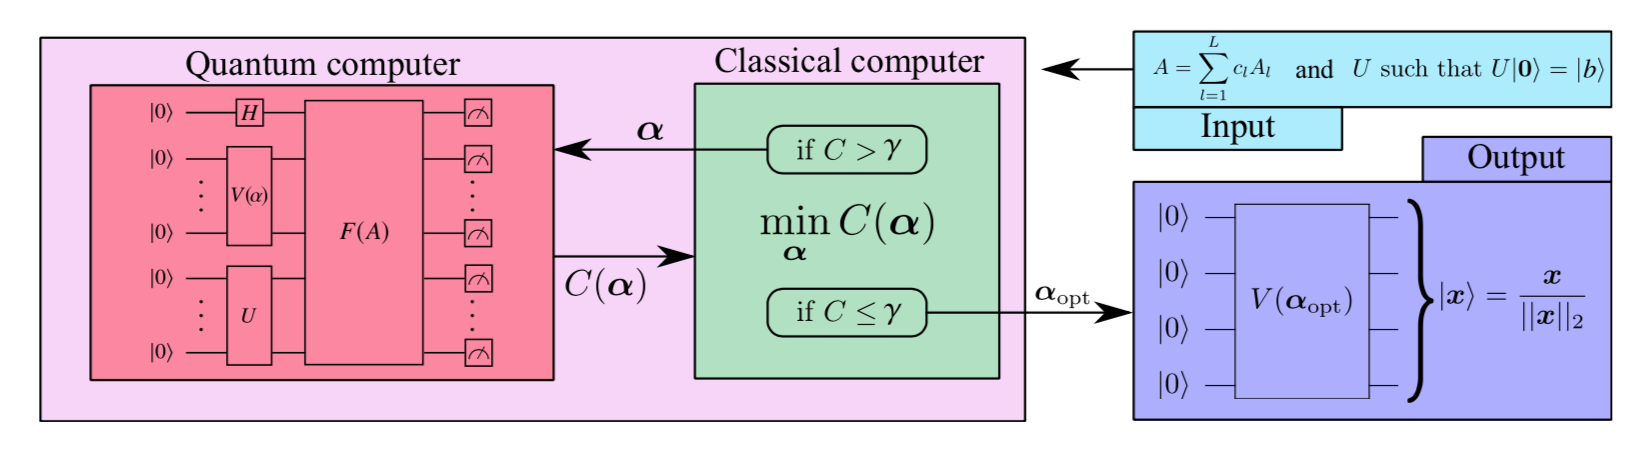
\includegraphics[scale=0.57]{bro.png}
   
    \caption{
        \justifying
        Scematic diagram of the VLQS algorithm. It illustrates the algorithm (light pink box) receiving as input the matrices ${\bf A} = \sum_{l = 1}^{L}c_lA_l$ and $U$ and returning the optimal parameters 
    $\boldsymbol{\alpha}_{opt}$ which produced the optimal solution $\ket{x}$. Inside the light pink box it is shown the interaction between the quantum circuit (left) and the classical circuit (right) as previously described.}
\end{figure}
{\raggedleft
\rule{\textwidth}{.5pt}}\\
\section*{{\bf Complexity of the VQLS}}
The cited paper provides numerical simulations for specific matrices $A$ with fixed conditioned number and with a particular precision. The result of those simulations proves that the algorithm achieves polynomial scaling in $n$ and therefore polylogarithmic scaling in $N$, since $N=2^n$.
Namely, to guarantee precision 0.3 with $n = 2, ..., 7$ and $condition\;number =10$, the obtained relation for the running time of the algorithm was $y \sim n^{8.5}$. Any further complexity analysis, other than the experimental one, is difficult due to the heuristic nature of the algorithm. The figure bellow (taken from the original paper) presents the simulation results 
\begin{figure}[H]
    
    \centering{
    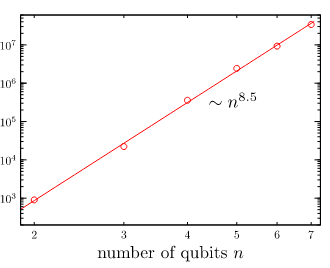
\includegraphics[scale=0.57]{Screenshot 2023-02-08 at 02-55-02 1909.05820.pdf.png}
    }
    \caption{
        \justifying
        Time-to-solution versus n needed to guarantee precision $= 0.3$. All matrices had a condition number $\kappa = 10$.}
\end{figure}
{\raggedleft
\rule{\textwidth}{.5pt}}\\
\section*{{\bf The Ansatz}}
The Ansatz is the oparator, responsible of preparing the state $\ket{x}$ when it acts on state $\ket{\bf 0}$. It should be capable of generating any arbitrary state on Hilbert space, including the entangled states.
A possible way of implementing such an oparator, is by employing single qubits rotation gates (such as $R_X, R_Y, R_Z$) for "exploring" the space alongside some two-qubit gates to provide the entanglement(such as $CX, CZ, CH$).
Each rotation gate should correspond to one of the parameters of ${\boldsymbol{\alpha}} = (\alpha_1,\alpha_2,...)$.
One could consider two possible implementation of the Ansatz. Firstly, the {\bf fixed-structure ansatz} in which the configuration of the gates remains the same throughout the execution of the algorithm and secondly, the {\bf variable-structure ansatz}
in which the gate's placement is changing. In this report we will focus only on the fixed stucture ansatz.\\
Two simple variations of the fixed structure ansatz are the following 
\begin{figure}[H]
    \[
    \begin{array}{c}
    
        \Qcircuit @C=0.7em @R=2em {
           & \qw& \gate{R_Y(a_1)} & \ctrl{1}& \qw & \qw &\qw &\gate{R_Y(a_5)} & \ctrl{1} &\qw & \qw &\qw\\
            &\qw&  \gate{R_Y(a_2)} & \targ &\ctrl{1}& \qw &\qw &\gate{R_Y(a_6)} & \targ & \ctrl{1} & \qw &\qw \\
            &\qw& \gate{R_Y(a_3)} & \qw &\targ & \ctrl{1}&\qw &\gate{R_Y(a_7)} & \qw & \targ & \ctrl{1}  &\qw\\
            &\qw& \gate{R_Y(a_4)} & \qw &\qw & \targ &\qw &\gate{R_Y(a_8)} & \qw & \qw & \targ  &\qw\\
            & & & & & &\mbox{(a)}\\
            }
    \end{array}
    \;\;\;\;\;\;\;\;
    \begin{array}{c}
    
        \Qcircuit @C=0.7em @R=2em {
           & \qw& \gate{R_Y(a_1)} & \ctrl{1}& \qw &\gate{R_Y(a_5)} &\qw &\qw\\
            &\qw&  \gate{R_Y(a_2)} & \targ &\ \qw &\gate{R_Y(a_6)} & \ctrl{1} &\qw\\
            &\qw& \gate{R_Y(a_3)} & \ctrl{1} &\qw &\gate{R_Y(a_7)} & \targ &\qw\\
            &\qw& \gate{R_Y(a_4)} & \targ &\qw&\gate{R_Y(a_8)} &\qw &\qw\\
            & & & &\mbox{(b)}\\
            } 
    
    \end{array}
    \]
    \caption{$R_Y$-$C_X$ ansatz for 4 qubits.$(a)$ linear entanglement $(b)$ alternating entanglement,}
    \end{figure} 

Note that in place of the $R_Y$ gates can be settled $R_X$ or $R_XR_Z$ or $R_XR_Y$ etc. and in place of $CX$ gates can be settled $CZ$ or $CH$. Furthermore it can be proved the order of the $CX$ gates does not matter.
One can observe that the two different circuits use the same number of effective parameters ($R_Y$ gates) but circuit $(b)$ uses half the number of $CX$ gates. Hence we consider the alternating entanglement 
ansatz as the optimal solution, since it is more efficient than the linear entanglement in terms of the number of effective parameters per two-qubit gate.\\
\rule{\textwidth}{.5pt}\\
\section*{{\bf The Cost function}}
As it was previously stated, the cost function needs to decrease as the state $\ket{\psi} = \ket{\psi(\boldsymbol{\alpha})}:={\bf A}\ket{x(\boldsymbol{\alpha})}$ tends to become proportional to $\ket{b}$ and increase as $\ket{\psi}$ and $\ket{b}$ are close to being orthogonal.
A suitable indicator that shows the overlap between $\ket{\psi}$ and $\ket{b}$ is their inner product $\braket{\psi|b}$. The general form of a cost function in VQA problems is: 
$$\hat{C}_G  = \braket{\psi|H_G|\psi}$$
A simple Hamiltonian $H_G$ to take advantage of the overlap, is $H_G=\mathbb{I} -\ket{b}\bra{b}$. Hence the cost funcion is:
$$\hat{C}_G  = \braket{\psi|(\mathbb{I} -\ket{b}\bra{b})|\psi}=\braket{\psi|\psi} - |\braket{b|\psi}|^2$$
which takes values within the set $\hat{C}_G \in [0,\braket{\psi|\psi}]$ (taking into account that $\ket{b}$ is normalized). However a potential $\ket{\psi}$ with small norm relative to the tolerance $\gamma$ 
could cause a premature termination of the algorithm, since the value of the cost function would be cosidered "small enough" at any point.

To tackle this issue, it is preferable to use a normalized version of this cost function 
$$C_G = \frac{\hat{C}_G}{\braket{\psi|\psi}}=1 - \frac{|\braket{b|\psi}|^2}{\braket{\psi|\psi}} $$

\subsection*{Global and Local cost function}
If we proceed to write $C_G$ more explicitly, using that $\ket{b} = U\ket{\bf 0}$ and $\ket{\psi} = {\bf A}\ket{x} = \sum_{l = 1}^{L}c_lA_lV({\boldsymbol{\alpha}})\ket{\bf 0}$, then we end up having the following expression:
\begin{align*}
    C_G &= 1 - \frac{\braket{\psi|b}\braket{b|\psi}}{\braket{\psi|\psi}} = 1 - \frac{\left(\sum_{l = 1}^{L}c_l^* \bra{\bf 0}V^\dag({\boldsymbol{\alpha}})A_l^\dag U\ket{\bf 0}\right)\left(\sum_{l = 1}^{L}c_l \bra{\bf 0}U^\dag A_lV({\boldsymbol{\alpha}})\ket{\bf 0}\right)}
    {\left(\sum_{l = 1}^{L}c_l^* \bra{\bf 0}V^\dag({\boldsymbol{\alpha}})A_l^\dag \right)\left(\sum_{l = 1}^{L}c_l  A_lV({\boldsymbol{\alpha}})\ket{\bf 0}\right)} =\\ \\
    &=  1 - \frac{\sum_{l = 1}^{L}\sum_{l' = 1}^{L}c_{l'} c_l^* \bra{\bf 0}V^\dag({\boldsymbol{\alpha}})A_l^\dag U\ket{\bf 0}\bra{\bf 0}U^\dag A_{l'}V({\boldsymbol{\alpha}})\ket{\bf 0}}
    {\sum_{l = 1}^{L}\sum_{l' = 1}^{L}c_{l'} c_l^* \bra{\bf 0}V^\dag({\boldsymbol{\alpha}})A_l^\dag  A_{l'}V({\boldsymbol{\alpha}})\ket{\bf 0}}
\end{align*}\\
The above is called {\bf global cost function} and even though it works fine in most of the cases, it can still be vulnerable to barren plateaus\footnote{Barren plateau landscapes correspond to gradients that vanish exponentially in the number of qubits. In other words barren plateau describes a situation where the cost function landscape is flat and its gradient is almost 0, which prevents the optimization algorithm from making significant progress arround that area}
when it comes to a large number of qubits ($n\approx 50$).
For this reason, an alternative cost funcion has been proposed, the {\bf local cost function }:
$$\textnormal{The local Hamiltonian is:  } H_L = \mathbb{I}- \frac{1}{n}\sum_{j=1}^{n}\ket{0_j}\bra{0_j}\otimes\mathbb{I}_{\overline{j}}$$
\begin{align*}
    C_L &=  1 - \frac{\sum_{l = 1}^{L}\sum_{l' = 1}^{L}c_{l'} c_l^* \bra{\bf 0}V^\dag({\boldsymbol{\alpha}})A_l^\dag U\left(\frac{1}{n}\sum_{j=0}^{n-1}(\ket{0_j}\bra{0_j}\otimes \mathbb{I}_{\overline j} )\right)U^\dag A_{l'}V({\boldsymbol{\alpha}})\ket{\bf 0}}
    {\sum_{l = 1}^{L}\sum_{l' = 1}^{L}c_{l'} c_l^* \bra{\bf 0}V^\dag({\boldsymbol{\alpha}})A_l^\dag  A_{l'}V({\boldsymbol{\alpha}})\ket{\bf 0}} = \\ \\
    & = 1 -\frac{1}{n} \frac{\sum_{l = 1}^{L}\sum_{l' = 1}^{L}\sum_{j=0}^{n-1}c_{l'} c_l^* \bra{\bf 0}V^\dag({\boldsymbol{\alpha}})A_l^\dag U(\ket{0_j}\bra{0_j}\otimes \mathbb{I}_{\overline j} )U^\dag A_{l'}V({\boldsymbol{\alpha}})\ket{\bf 0}}
    {\sum_{l = 1}^{L}\sum_{l' = 1}^{L}c_{l'} c_l^* \bra{\bf 0}V^\dag({\boldsymbol{\alpha}})A_l^\dag  A_{l'}V({\boldsymbol{\alpha}})\ket{\bf 0}}
\end{align*}\\
With $\ket{0_j}\bra{0_j}$ being the projection operator $\ket{0}\bra{0}$ applyed on qubit $j$ and $\mathbb{I}_{\overline j}$ the identity on all qubits except $j$. Essentially, $\ket{\bf 0}\bra{\bf 0}$
has been replaced with $\frac{1}{n}\sum_{j=0}^{n-1}(\ket{0_j}\bra{0_j}\otimes \mathbb{I}_{\overline j})$. Now instead of applying the cost function across all qubits (which is why barren plateaus occur) we have  divided the problem up into multiple single-qubit terms, and summed all the results up.

It needs to be confirmed now, that the local cost function is indeed valid for our problem. It can be proved That
$$C_L \leq C_G \leq nC_L $$ 
which suggests that when $C_G \rightarrow 0 $ so does the $C_L$. The same is true for the opposite way, when $C_L \rightarrow 0 $ so does the $C_G$. This alone is enough to approve $C_L$ for our purpose.
\subsection*{Evaluation of the cost function using quantum circuit}
As it has already been mentioned, the algorithm requires a quantum circuit to receive as input the parameters $\boldsymbol{\alpha}$ and return the value of the cost function on point $\boldsymbol{\alpha}$, $C_G(\boldsymbol{\alpha})$
(or $C_L(\boldsymbol{\alpha})$). Having defined our two different cost functions, we are left with the task of calculating the following quantities:
\begin{itemize}
    \item if we use the global cost funtion we need to calculate the terms:
    $$\beta_{ll'} =  \bra{\bf 0}V^\dag({\boldsymbol{\alpha}})A_l^\dag  A_{l'}V({\boldsymbol{\alpha}})\ket{\bf 0}$$
    and
    $$\gamma_{ll'} =  \bra{\bf 0}V^\dag({\boldsymbol{\alpha}})A_l^\dag U\ket{\bf 0}\bra{\bf 0}U^\dag A_{l'}V({\boldsymbol{\alpha}})\ket{\bf 0}$$
    \item whereas, if we wish to use the local cost function the terms are:
    $$\beta_{ll'} =  \bra{\bf 0}V^\dag({\boldsymbol{\alpha}})A_l^\dag  A_{l'}V({\boldsymbol{\alpha}})\ket{\bf 0}$$
    and
    $$\delta_{ll'}^{(j)}= \bra{\bf 0}V^\dag({\boldsymbol{\alpha}})A_l^\dag U(\ket{0_j}\bra{0_j}\otimes \mathbb{I}_{\overline j} )U^\dag A_{l'}V({\boldsymbol{\alpha}})\ket{\bf 0}$$
    
\end{itemize}
The latter ($\delta_{ll'}^{(j)}$), can be rewritten more conviniently by noticing that $\ket{0_j}\bra{0_j} = \frac{1}{2}(\mathbb{I}_{j} + Z_j)$\footnote[1]{$Z_j$ indicates the operator $Z$ applyed on qubit $j$}. 
The reformed term will be :
\begin{align*}
    \delta_{ll'}^{(j)}&= \bra{\bf 0}V^\dag({\boldsymbol{\alpha}})A_l^\dag U\left(\frac{1}{2}(\mathbb{I}_{j} + Z_j)\otimes \mathbb{I}_{\overline j} \right)U^\dag A_{l'}V({\boldsymbol{\alpha}})\ket{\bf 0} =\\
    & = \frac{1}{2}\bra{\bf 0}V^\dag({\boldsymbol{\alpha}})A_l^\dag UU^\dag A_{l'}V({\boldsymbol{\alpha}})\ket{\bf 0} + \frac{1}{2}\bra{\bf 0}V^\dag({\boldsymbol{\alpha}})A_l^\dag U(Z_j\otimes \mathbb{I}_{\overline j} )U^\dag A_{l'}V({\boldsymbol{\alpha}})\ket{\bf 0} = \\
    &\stackrel{\textnormal{\footnotemark}}{=}  \frac{1}{2}\bra{\bf 0}V^\dag({\boldsymbol{\alpha}})A_l^\dag  A_{l'}V({\boldsymbol{\alpha}})\ket{\bf 0} + \frac{1}{2}\bra{\bf 0}V^\dag({\boldsymbol{\alpha}})A_l^\dag U(Z_j\otimes \mathbb{I}_{\overline j} )U^\dag A_{l'}V({\boldsymbol{\alpha}})\ket{\bf 0} = \\
    & = \frac{1}{2}\beta_{ll'} + \frac{1}{2}\bra{\bf 0}V^\dag({\boldsymbol{\alpha}})A_l^\dag U(Z_j\otimes \mathbb{I}_{\overline j} )U^\dag A_{l'}V({\boldsymbol{\alpha}})\ket{\bf 0}
\end{align*}
or equivalently, the factor $\frac{1}{2}$ can be ignored:
$$\delta_{ll'}^{(j)} = \beta_{ll'} + \bra{\bf 0}V^\dag({\boldsymbol{\alpha}})A_l^\dag U(Z_j\otimes \mathbb{I}_{\overline j} )U^\dag A_{l'}V({\boldsymbol{\alpha}})\ket{\bf 0}$$
\footnotetext{since $U$ is unitary $UU^\dag = \mathbb{I}$}
\subsubsection*{The Hadamard Test}
In order to calculate terms similar to the ones above, we employ a quantum circuit called the Hadamard test. \\

\begin{figure}[h]


    \[
    \begin{array}{c}
    
        \Qcircuit @C=2em @R=2em {
            \lstick{\ket{0}} &\gate{H} & \ctrl{1} & \gate{H} &\meter & \cw \\
            \lstick{\ket{\psi}} & {/}^n\qw & \gate{U_H} &  \qw & \qw
            }
    
    \end{array}
    \]
    \caption{The Hadamard Test. Calculates the Real part of the expected value of $U_H$ with respect to state $\ket{\psi}$}
    \end{figure}
    The Hadamard test in Figure 4 can be used to calculate the term $\textnormal{Re}\left[\braket{\psi|U_H|\psi}\right]$, where $U_H$ is some unitary operator and $\ket{\psi}$ is an arbitrary state.
    The first qubit used to control the $U_H$ is called the {\bf achilla} and if it is mesured, the probability of being 0 is $\frac{1}{2}(1+\textnormal{Re}\left[\braket{\psi|U_H|\psi}\right])$
    and the probability of being 1 is $\frac{1}{2}(1-\textnormal{Re}\left[\braket{\psi|U_H|\psi}\right])$. Their difference is 
    $$P(0) - P(1) =  \frac{1}{2}(1+\textnormal{Re}\left[\braket{\psi|U_H|\psi}\right]) - \frac{1}{2}(1-\textnormal{Re}\left[\braket{\psi|U_H|\psi}\right]) = \textnormal{Re}\left[\braket{\psi|U_H|\psi}\right]$$
    For the sake of completeness, the proof is the following:
    \begin{align*}
        &\ket{0}\otimes\ket{\psi} \xrightarrow{H \textnormal{ on first bit}} \frac{1}{\sqrt{2}}(\ket{0}\otimes\ket{\psi} + \ket{1}\otimes\ket{\psi}) 
         \xrightarrow{\textnormal{applying control } U_H} \frac{1}{\sqrt{2}}(\ket{0}\otimes\ket{\psi} + \ket{1}\otimes U_H\ket{\psi})\\
         & \xrightarrow{H \textnormal{ on first bit}} \frac{1}{{2}}(\ket{0}\otimes\ket{\psi} + \ket{1}\otimes\ket{\psi}+\ket{0}\otimes U_H\ket{\psi}-\ket{1}\otimes U_H\ket{\psi})\\
         &= \frac{1}{{2}}(\ket{0}\otimes(\mathbb{I} + U_H)\ket{\psi} + \ket{1}\otimes(\mathbb{I} - U_H)\ket{\psi})
    \end{align*}
    Thus 
    \begin{align*}
        P(0) &= \frac{1}{4}\bra{\psi}(\mathbb{I} + U_H)(\mathbb{I} + U_H^\dag)\ket{\psi} = \frac{1}{4}\bra{\psi}(\mathbb{I}^2+ U_H + U_H^\dag +U_HU_H^\dag)\ket{\psi}=\\
        & = \frac{1}{4}\bra{\psi}(2\mathbb{I}+ U_H + U_H^\dag )\ket{\psi}=\frac{1}{4}\left(2\bra{\psi}\mathbb{I}\ket{\psi}+ \bra{\psi}U_H\ket{\psi} + \bra{\psi}U_H^\dag\ket{\psi} \right) =\\
        & = \frac{1}{4}\left(2+ \bra{\psi}U_H\ket{\psi} + (\bra{\psi}U_H^\dag\ket{\psi})^* \right) = \frac{1}{2}(1+\textnormal{Re}\left[\braket{\psi|U_H|\psi}\right])
    \end{align*}
    $P(1)$ is calculated similarly\\ \\
    To obtain the Imaginary part, we simple add a $S^\dag$ after the first hadamard gate on the ancilla qubit
    \begin{figure}[h]


        \[
        \begin{array}{c}
        
            \Qcircuit @C=2em @R=2em {
                \lstick{\ket{0}} &\gate{H} & \gate{S^\dag}  &\ctrl{1} & \gate{H} &\meter & \cw \\
                \lstick{\ket{\psi}} & {/}^n\qw & \qw &\gate{U_H} &  \qw & \qw
                }
        
        \end{array}
        \]
        \caption{The Hadamard Test. Calculates the Imaginary part of the expected value of $U_H$ with respect to state $\ket{\psi}$}
        \end{figure}
        \begin{align*}
            &\ket{0}\otimes\ket{\psi} \xrightarrow{H \textnormal{ on first bit}} \frac{1}{\sqrt{2}}(\ket{0}\otimes\ket{\psi} + \ket{1}\otimes\ket{\psi}) 
            \xrightarrow{S^\dag \textnormal{ on first bit}} \frac{1}{\sqrt{2}}(\ket{0}\otimes\ket{\psi} -i \ket{1}\otimes\ket{\psi})\\
            & \xrightarrow{\textnormal{applying control } U_H} \frac{1}{\sqrt{2}}(\ket{0}\otimes\ket{\psi} -i \ket{1}\otimes U_H\ket{\psi})\\
             & \xrightarrow{H \textnormal{ on first bit}} \frac{1}{{2}}(\ket{0}\otimes\ket{\psi} + \ket{1}\otimes\ket{\psi}-i\ket{0}\otimes U_H\ket{\psi}+i\ket{1}\otimes U_H\ket{\psi})\\
             &= \frac{1}{{2}}(\ket{0}\otimes(\mathbb{I} -i U_H)\ket{\psi} + \ket{1}\otimes(\mathbb{I} +i U_H)\ket{\psi})
        \end{align*}
        Thus 
    \begin{align*}
        P(0) &= \frac{1}{2}(1+\textnormal{Im}\left[\braket{\psi|U_H|\psi}\right])
    \end{align*}
    Same procedure for $P(1)$ \\ \\

    Having explained the functionality of the Hadamard test, what remains to be seen how to make use of it in order to compute the terms of the VLQS ploblem, starting off with the terms $\beta_{ll'}$.

    $$\beta_{ll'} =  \bra{\bf 0}V^\dag({\boldsymbol{\alpha}})A_l^\dag  A_{l'}V({\boldsymbol{\alpha}})\ket{\bf 0}$$
    By setting $\ket{\psi} = V({\boldsymbol{\alpha}})\ket{\bf 0}$ and  $ U_H = A_l^\dag  A_{l'}$, we obtain that $\beta_{ll'} = \braket{\psi|U_H|\psi}$ which is similar to the Hadamard test form.
    Hence $\beta_{ll'}$ can be calculated using the circuit bellow:

    \begin{figure}[H]


        \[
        \begin{array}{c}
        
            \Qcircuit @C=2em @R=2em {
                \lstick{\ket{0}} &\gate{H} & \gate{S^\dag}  &\ctrl{1} & \ctrl{1}&\gate{H} &\meter & \cw \\
                \lstick{\ket{0}} & {/}^n\qw & \gate{V({\boldsymbol{\alpha}})} &\gate{A_{l'}} & \gate{A_l^\dag}&  \qw & \qw \gategroup{1}{3}{1}{3}{.7em}{--}
                \
                }
        
        \end{array}
        \]
        \caption{The Hadamard Test for evaluating the terms $\beta_{ll'}=  \bra{\bf 0}V^\dag({\boldsymbol{\alpha}})A_l^\dag  A_{l'}V({\boldsymbol{\alpha}})\ket{\bf 0}$. The $S^\dag$ gate in dashed box indicates, the gate's involvment only when calculating the Imaginary part of $\beta_{ll'}$.}
        \end{figure}
        In succesion, if we proceed we the the global cost function we have to evaluate the terms 
        $$ \gamma_{ll'} =  \bra{\bf 0}V^\dag({\boldsymbol{\alpha}})A_l^\dag U\ket{\bf 0}\bra{\bf 0}U^\dag A_{l'}V({\boldsymbol{\alpha}})\ket{\bf 0}$$
        which can be accomplished in three different ways:
        \begin{itemize}
            \item The terms $\bra{\bf 0}V^\dag({\boldsymbol{\alpha}})A_l^\dag U\ket{\bf 0}$ and $\bra{\bf 0}U^\dag A_{l'}V({\boldsymbol{\alpha}})\ket{\bf 0}$ will be evaluated separately by using two different 
            Hadamard Tests with the $\ket{\psi} = \ket{0}$ and by controlling each one of the inner unitaries

        \end{itemize} 
        \begin{figure}[H]
        \[
        \begin{array}{c}
        
            \Qcircuit @C=0.7em @R=2em {
                \lstick{\ket{0}} &\gate{H} & \gate{S^\dag}  &\ctrl{1} & \ctrl{1} & \ctrl{1} &\gate{H} &\meter & \cw \\
                \lstick{\ket{0}} & {/}^n\qw &  \qw & \gate{U} &\gate{A_l^\dag} & \gate{V({\boldsymbol{\alpha}})^\dag}&  \qw & \qw \gategroup{1}{3}{1}{3}{.7em}{--}\\
                & & & & \mbox{(a)}\\
                }
        
        \end{array}
        \;\;\;\;\;\;\;\;
        \begin{array}{c}
        
            \Qcircuit @C=0.7em @R=2em {
                \lstick{\ket{0}} &\gate{H} & \gate{S^\dag}  &\ctrl{1} & \ctrl{1} & \ctrl{1} &\gate{H} &\meter & \cw \\
                \lstick{\ket{0}} & {/}^n\qw &  \qw &  \gate{V({\boldsymbol{\alpha}})} &\gate{A_{l'}} & \gate{U^\dag}&  \qw & \qw \gategroup{1}{3}{1}{3}{.7em}{--}\\
                & & & & \mbox{(b)}\\
                }
        
        \end{array}
        \]
        \caption{Two different Hadamard Tests for evaluating the terms $\bra{\bf 0}V^\dag({\boldsymbol{\alpha}})A_l^\dag U\ket{\bf 0}$ (circuit $(a)$ on the left) and  $\bra{\bf 0}U^\dag A_{l'}V({\boldsymbol{\alpha}})\ket{\bf 0}$ (circuit $(b)$ on the right)}
        \end{figure}
        \begin{itemize}
            \item For the second way, we write the second term as  
            $$ \bra{\bf 0}V^\dag({\boldsymbol{\alpha}})A_l^\dag U\ket{\bf 0}= (\bra{\bf 0}U^\dag A_{l}V({\boldsymbol{\alpha}})\ket{\bf 0})^\dag = (\bra{\bf 0}U^\dag A_{l}V({\boldsymbol{\alpha}})\ket{\bf 0})^* $$
            Thus, instead of using two different Hadamard Tests, it is only required to use the first one (Figure 7 circuit $(b)$) twice.
            \item The thrid method, wich is probably the optimal one, is using a different  subroutine called the {\bf Hadamard-Overlap Test}. Its advantage over the method with the regular Hadamard Test is that it doesn't require to control the ansazt or the $U$ at the expense of using $2n+1$ qubits onstead of $n+1$.
            Further explanation of the Hadamard-Overlap Test will not be held in this report
        \end{itemize} 
        Alternatly if we proceed with the local cost function we have to evaluate the terms 
        $$\delta_{ll'}^{(j)} = \beta_{ll'} + \bra{\bf 0}V^\dag({\boldsymbol{\alpha}})A_l^\dag U(Z_j\otimes \mathbb{I}_{\overline j} )U^\dag A_{l'}V({\boldsymbol{\alpha}})\ket{\bf 0}$$
        For the Hadamard Test of this term evaluation we set
        
        $$\ket{\psi} = V({\boldsymbol{\alpha}})\ket{\bf 0} \;\;\textnormal{ and } \;\;U_H = A_l^\dag U(Z_j\otimes \mathbb{I}_{\overline j} )U^\dag A_{l'}$$ 
        \begin{figure}[H]
            \[
            \begin{array}{c}
            
                \Qcircuit @C=1.7em @R=2em {
                    \lstick{\ket{0}} &\gate{H} & \gate{S^\dag}  &\ctrl{1} & \qw & \ctrl{1}&\qw & \ctrl{1}&\gate{H} &\meter & \cw \\
                    \lstick{\ket{0}} &\multigate{2}{V({\boldsymbol{\alpha}})} &\qw & \multigate{2}{A_l}  &\multigate{2}{U^\dag} & \gate{Z} & \multigate{2}{U} & \multigate{2}{A_{l'}^\dag}  & \qw & \qw \\
                    \lstick{\vdots}  & & & & & \vdots & & & &\rstick{\vdots}   \\
                    \lstick{\ket{0}} & \ghost{V({\boldsymbol{\alpha}})} &\qw & \ghost{A_l}  &\ghost{U^\dag} & \qw & \ghost{U} & \ghost{A_{l'}^\dag}   \qw & \qw & \qw \gategroup{1}{3}{1}{3}{.7em}{--}
                    }
            
            \end{array}
            \]
            \caption{The Hadamard Test for evaluating the terms $\delta_{ll'}^{(j)} = \beta_{ll'} + \bra{\bf 0}V^\dag({\boldsymbol{\alpha}})A_l^\dag U(Z_j\otimes \mathbb{I}_{\overline j} )U^\dag A_{l'}V({\boldsymbol{\alpha}})\ket{\bf 0}$.}
            \end{figure}
One can notice that the operators $U$ and  $U^\dag$ do not need to be controlled. This is because if the ancilla bit is $0$ the operator $Z_j\otimes \mathbb{I}_{\overline j} $ will not apply and therefore $U$ and $U^\dag$ will act successivly.
But since $U$ is unitary $UU^\dag = \mathbb{I}$. Thus, it makes no difference whether we control them or not.\\
\rule{\textwidth}{.5pt}\\
\section*{Qiskit Implementation}
Using the theoritical analysis above, we proceed to implement the VQLS algorithm in qiskit. The algorithm should solve the 3-qubits linear equations system
${\bf Ax=b}$ where 
$${\bf A} = 0.4 H_2 + 0.3Z_1+0.3X_3 \;\;\textnormal{  and  } \;\;\ket{b} = H_1\otimes H_2\otimes H_3 \ket{\bf 0}$$
For the ansatz we have chosen a circuit similar to the one in Figure 3 $(a)$. Even though we explained that the circuit with alternating entanglement is more efficient than the one with the linear entanglement,
 for the 3-qubits case, an alternating entanglement circuit like the following 
\begin{figure}[H]
    \[
    \begin{array}{c}
    
        \Qcircuit @C=0.7em @R=0.8em {
           & \qw& \gate{R_Y(a_1)} & \ctrl{1}& \qw &\gate{R_Y(a_5)} &\qw &\qw\\
            &\qw&  \gate{R_Y(a_2)} & \targ &\ \qw &\gate{R_Y(a_6)} & \ctrl{1} &\qw\\
            &\qw& \gate{R_Y(a_3)} & \qw &\qw &\gate{R_Y(a_7)} & \targ &\qw
            } 
    
    \end{array}
    \]
    \end{figure} 
would reduce the number of effective parameters ($a_3$ and $a_7$ would count as one parameter). So the implemented ansatz is
\begin{figure}[H]
    
    \centering
    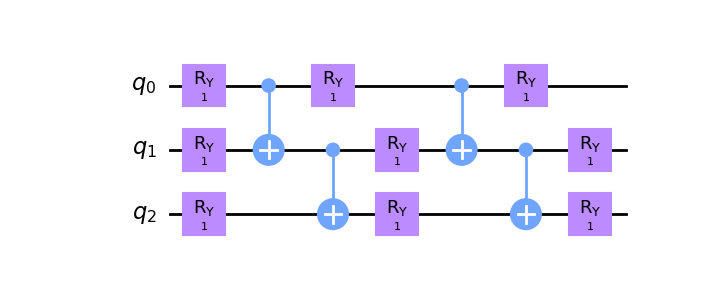
\includegraphics[scale=0.8]{Figure_1.png}
   
    \caption{
        \justifying
        Linear entanglement ansatz implemented in qiskit with 9 effective parameters (all initialized at 1) and 4 CNOTs gates. Since $\bf A$ and $\ket{b}$ are real, only rotation around the y-axis is required}
\end{figure}

For the cost function we use the global cost function and the terms $\gamma_{ll'}$ are evaluated with the second method that was described above (Figure 7 $(b)$).
\begin{figure}[H]
    
    \centering
    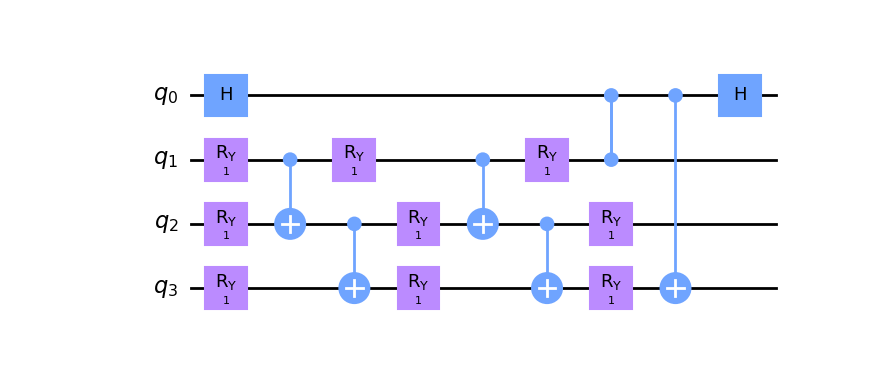
\includegraphics[scale=0.6]{Figure_2.png}
   
    \caption{
        \justifying
        \centering
        Hadamard Test for evaluating the terms $\beta_{ll'}$. With $A_l = Z_1$ and $A_{l'} = X_3$}
\end{figure}    

\begin{figure}[H]
    
    \centering
    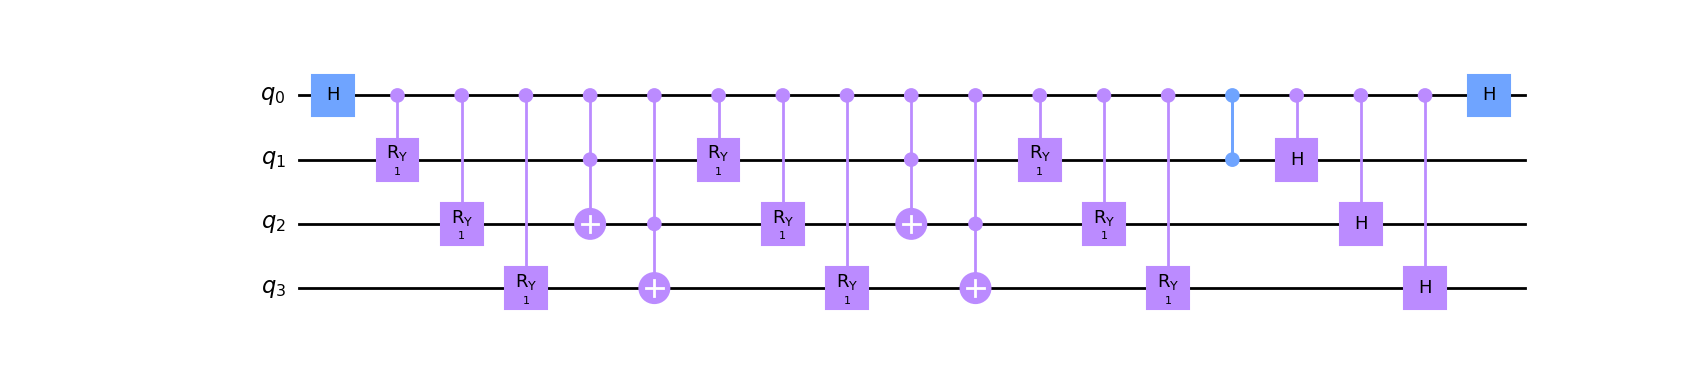
\includegraphics[scale=0.4]{Figure_3.png}
   
    \caption{
        \justifying
        \centering
        Hadamard Test for evaluating the terms $\gamma_{ll'}$. With $A_l = Z_1$ }
\end{figure} 

Note how in the last circuit, $U$ and $V({\boldsymbol{ \alpha}})$ are also controlled alongside $A_l$. The eventual cost function is :
 $$ C_G = 1 - \frac{\sum_{l = 1}^{L}\sum_{l' = 1}^{L}c_{l'} c_l^* \gamma_{ll'}}
 {\sum_{l = 1}^{L}\sum_{l' = 1}^{L}c_{l'} c_l^* \beta_{ll'}} $$\\
Our goal is to minimize it until it reaches the value $0$. To do so we employ the COBYLA optimizer which is gradient-free. Since we used the global cost function, a gradient-free optimizer 
is convinient because it is less impacted by barren plateaus. The final result of the optimization process is the following:\\ \\ \\  
\begin{verbatim}
      fun: 0.00012637933571213456
    maxcv: 0.0
  message: 'Maximum number of function evaluations has been exceeded.'
     nfev: 200
   status: 2
  success: False
        x: array([ 3.31224364,  1.54576436,  4.69185342, -0.94657516,  1.98048994,
         0.04202637,  0.11539815,  2.38380735,  3.18573665])
\end{verbatim}
\verb{fun{ is the final value of the cost function which is close to $0$, as desired. 
\verb{x{ is the optimal point $\boldsymbol{\alpha}_{opt} $ which corresponds to the solution $\ket{x} = V(\boldsymbol{\alpha}_{opt})\ket{\bf 0}$ .
Finally, we attempt to confirm that the obtained solution $\ket{x}$ is valid, by calculating the inner product $\braket{x{\bf A}|b}$ and expecting it to be $1$ 
\begin{verbatim}
    <xA|b> = (0.9998736206641057-0j)
\end{verbatim}    
As we can see, it is indeed close to $1$ with a very low deviation.

\section*{Referances}
\subsubsection*{VQLS Algorithm}
\url{https://arxiv.org/pdf/1909.05820.pdf}\\
\url{https://qiskit.org/textbook/ch-paper-implementations/vqls.html}\\
\url{https://pennylane.ai/qml/demos/tutorial_vqls.html}

\subsubsection*{Ansatz}
\url{https://arxiv.org/pdf/2111.13730.pdf}

\subsubsection*{Cost Function}
\url{https://pennylane.ai/qml/demos/tutorial_local_cost_functions.html}
\end{document}